%!TEX root = ../thesis.tex
%*******************************************************************************
%****************************** Introduction Chapter ***************************
%*******************************************************************************
\chapter{Background}

This thesis will focus on graph genome methods and their application to bacterial genomes. We pay particular attention to \mtb{} and \ont{} for our applications. i.e., why are we focusing on these particular topics in the background section?

% =============================================
\section{Bacterial genomes}
% Describe the concept of a bacterial pan-genome
% Describe some of the unique organisational elements of bacterial genomes - i.e., HGT, MGEs, recombination etc.
% How are pan-genomes analysed
% Variant calling in bacterial genomes
% Use the variant calling section to segway into graph genomes?
\subsection{Causes of bacterial diversity}
Bacteria have incredibly flexible genomes. The mechanisms of variation can be grouped into \emph{vertical} or \emph{horizontal} inheritance. Vertical inheritance is the passing of genetic material from parent to child during replication, while horizontal inheritance describes the acquisition of genetic information between cells without such an ancestor relationship. 

Vertically inherited variation generally consists of point mutations, insertions and deletions (indels), and structural rearrangements. Such mutations can arise due to a multitude of reasons: homologous recombination, DNA deamination, replication-transcript conflict, and replication errors to name a few \cite{Lan2000}. However, the dominant form of genomic variability in bacteria is horizontal inheritance \cite{McInerney2017}.

Horizontal inheritance operates via three main mechanisms - \textit{transduction}, \textit{conjugation}, and \textit{transformation} (or competence) - and are illustrated in \autoref{fig:horizontal-inheritance}.

\textit{Transduction} is mediated by bacteriophages (phages) - viruses which infect bacteria and are the most abundant organism on Earth \cite{mcgrath2007bacteriophage}. During phage propagation, parts of the host (bacteria) DNA can become encapsulated in the virus. If a phage goes on the infect another cell and eject this encapsulated DNA (transduction), it can recombine into the chromosome or begin replicating as a plasmid \cite{Chiang2019}. When the transduced DNA is a gene imparts a new, beneficial function, it can have obvious impacts on the recipient's evolution.

\textit{Conjugation} is the cell-to-cell transfer of DNA. A donor cell contacts another via a pilus and a copy of the DNA - normally a plasmid - is transmitted \cite{Soucy2015}. A more rare form of conjugation can occur when a plasmid has become incorporated into the chromosome of the donor (Hfr) and this portion of the chromosome is transferred to the recipient cell \cite{Redfield2001}.

\textit{Transformation} occurs when a cell interalises exogenous DNA, which in turn becomes incorporated into the chromosome by homologous recombination \cite{Johnston2014}. There is some debate about the exact purpose of transformation, with the general consensus being to increase genetic diversity; however, a nutritional role is also possible \cite{Johnston2014}.

\begin{figure}
\begin{center}
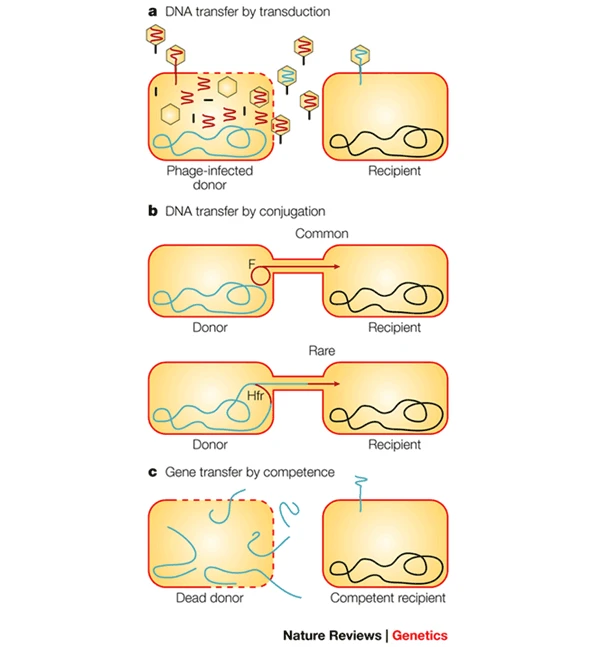
\includegraphics[width=0.95\columnwidth]{Chapter0/Figs/methods-of-dna-transfer.png}
\caption{{An illustration of the three main mechanisms of horizontal inheritance in bacteria. \textbf{a}) Transduction is facilitated by phages that encapsulate host DNA in one cell and eject that DNA into another cell. \textbf{b}) Conjugation, in its common form, is the transfer of a plasmid copy from a donor to a receiver cell via a pilus "bridge". In a rarer form, a plasmid that has been incorporated into the donor cell chromosome is transferred. \textbf{c}) Transformation (competence) is the uptake of exogenous DNA and subsequent incorporation into the chromosome.}
{\label{fig:horizontal-inheritance}}
}
\source{\cite{Redfield2001}}
\end{center}
\end{figure}

\noindent
These different means of inheritence conspire to create varying levels of diversity within bacterial species and give rise to the \textit{pan-genome}.

\subsection{The pan-genome}

A pan-genome is the full complement of genetic loci found within a given species. Traditionally, loci refer to genes, although we note that for the work we will describe in this thesis loci need not be genes.

The pan-genome can be broken into two subsets: the \textit{core} and \textit{accessory} genome. Loci that occur in the majority of species members are considered core, whilst everything else is deemed accessory (see \autoref{fig:pangenome-venn}). The accessory genome can be further broken down into intermediate and rare loci. 

The proportional size of the core genome varies dramatically between species. For instance, if we assume a gene is core if present in $\ge 95$\% of sampled species, the \textit{Escherichia coli} pan-genome is composed of 10\% core genes. Conversely, 89\% of the \textit{Mycobacterium tuberculosis} pan-genome is core genes (data was obtained from the panX database \cite{panx}). Species with a large pan-genome, such as \ecoli{}, have what is called an "open" pan-genome, while those with more conserved gene content, such as \mtb{}, are deemed "closed". 

Another interesting property of the bacterial genome is the distinctive "U-shaped" gene frequency distribution \cite{Lobkovsky2013,pandora,Lapierre2009}, shown in \autoref{fig:pangenome-freq}. This frequency distribution is a consequence of the fact that, in general, genes are either rare or common due to selective pressures \cite{Lobkovsky2013,thepangenome2020}. Moreover, the size of the bacterial pan-genome is estimated to be infinite \cite{Lapierre2009}, as hinted at by \autoref{fig:pangenome-size}.

\begin{figure}
     \centering
     \begin{subfigure}[b]{0.475\textwidth}
        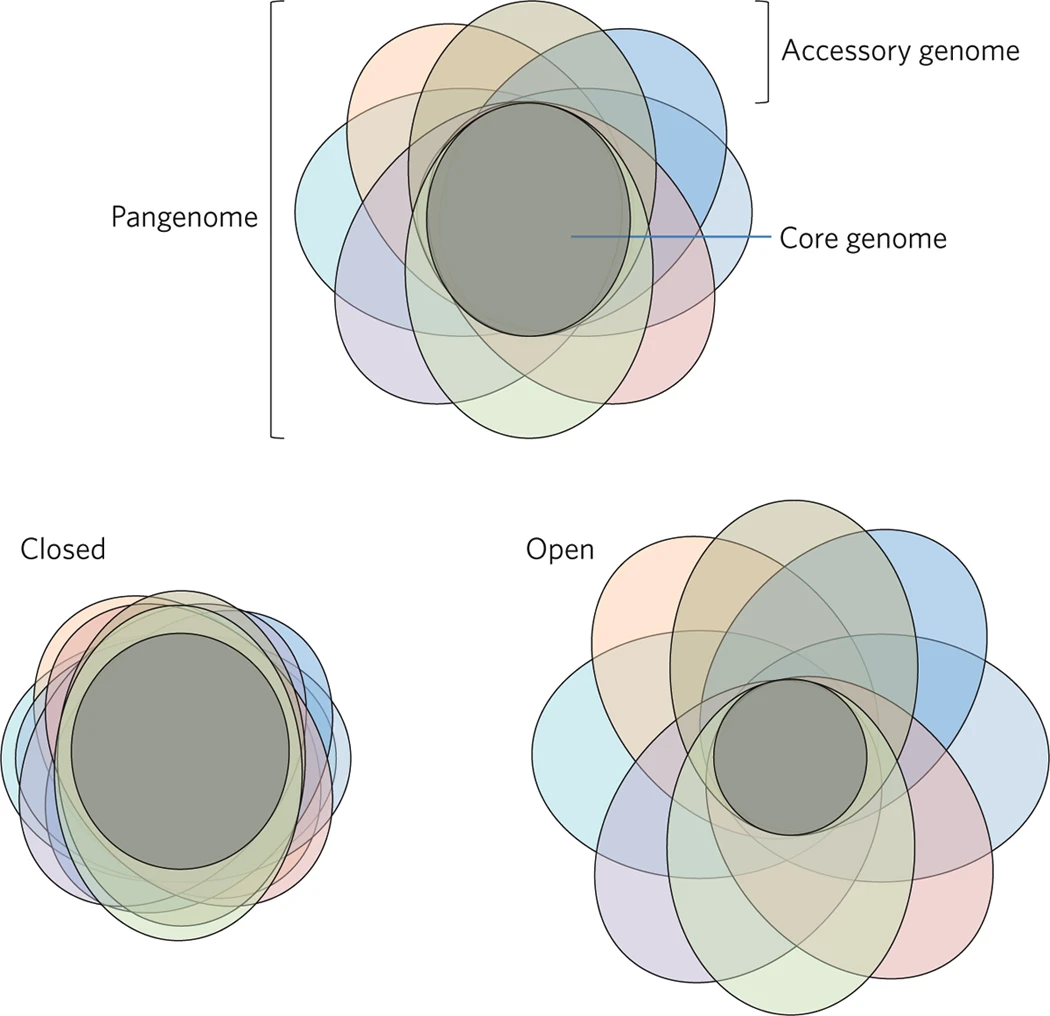
\includegraphics[height=0.21\textheight]{Chapter0/Figs/pangenome-venn.png}
        \centering
        \caption{}
        \label{fig:pangenome-venn}
        \source{\cite{McInerney2017}}
     \end{subfigure}
     \begin{subfigure}[b]{0.475\textwidth}
         \centering
        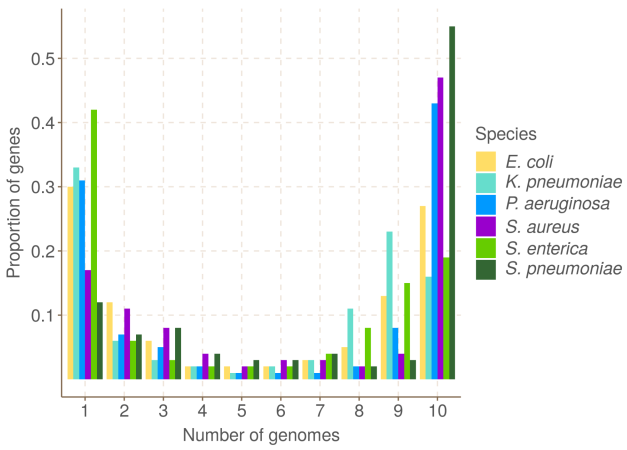
\includegraphics[height=0.21\textheight]{Chapter0/Figs/gene_frequency_distribution.png}
         \caption{}
         \label{fig:pangenome-freq}
         \source{\cite{pandora}}
     \end{subfigure}
     \begin{subfigure}[b]{0.8\textwidth}
        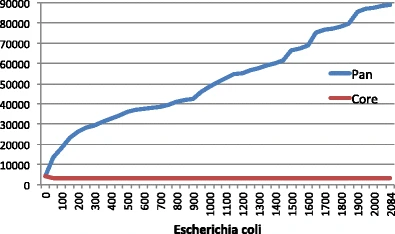
\includegraphics[width=1\linewidth]{Chapter0/Figs/pangenome-size.png}
        \centering
        \caption{}
        \label{fig:pangenome-size}
        \source{\cite{Land2015}}
     \end{subfigure}
    \caption{The size and gene frequency distribution of the bacterial pan-genome. \textbf{a}) Venn diagram representation of the pan-genome and its core and accessory components. \textbf{b}) The asymmetric U-shaped gene frequency distribution for 10 genomes within 6 bacterial species. Genes are generally rare (left) or common (right). \textbf{c}) the size (y-axis) of the core (red) and accessory (blue; Pan) genome of \ecoli{} as more genomes are sampled (x-axis).}
        \label{fig:pangenome}
\end{figure}

\noindent
These definitions of the pan-genome components (core and accessory) are somewhat simplistic. Recent work by Horesh \etal{} has highlighted that these traditional definitions are biased by lineage sampling \cite{Horesh2021}. As an example, we have a collection of 100 genomes, with 50 being from the same lineage ($L_1$). Let us say gene \textit{abc} occurs in all 50 members of $L_1$, but none of the other 50 genomes. Under the traditional pan-genomic definitions, we would call \textit{abc} an intermediate gene. However, if we gathered a further 1,000 genomes, none of which are lineage $L_1$, \textit{abc} would now be considered rare. In the new pan-genome model proposed by Horesh \etal{}, loci are given a classification that is structure-aware. The \textit{abc} gene from the example would be classified as lineage-specific core. Other categories include multi-lineage and collection core, along with the same categories for intermediate, rare, and a new varied frequency class. The collection core is analogous to the traditional core, with everything else being the accessory genome - albeit with a much finer level of detail.

\subsection{How are pan-genomes analysed?}

Most pan-genomic analyses of bacterial collections follow a similar approach: align the genomes with a tool such as Parsnp \cite{Treangen2014} or Rory \cite{Page2015}, extract the core genome alignments and either ignore the accessory genome or just produce a presence-absence matrix of it \cite{Arnold2018,Azarian2018,McNally2016,thepangenome2020}. When the accessory genome is investigated at the nucleotide level, it is generally focused on a small subset of genes related to specific phenotypes such as antimicrobial resistance (AMR; \cite{Boolchandani2019}) or virulence \cite{Vasquez2019}. As we have seen, the pan-genome size varies significantly, so depending on the species, such approaches could be "ignoring" large portions of the full genomic repertoire. Despite this, we have learned an enormous amount about bacteria and their pan-genomes with these methods.

\subsection{Variant calling of bacterial genomes}

A common (pan-)genomic analysis requirement, and a major focus of this thesis, is variant calling. However, depending on the application, this can be done in a number of different ways. For example, when characterising an outbreak, common approaches are to use a reference genome of the same, or very close, strain to the outbreak \cite{Taylor2015}, or assemble each sample and select the closest reference to it based on some typing strategy \cite{Wyres2021}. Alternatively, a reference-free approach can alleviate some of the reference bias induced when selecting a genome to call variants against and provide better resolution of an outbreak \cite{Cremers2020}.

Given the importance of bacterial variant calling to this thesis, we will briefly outline various approaches to calling variants in bacterial genomes and highlight their strengths and limitations.

\subsubsection{Alignment-based methods}

Alignment-based variant calling also assumes a reference genome is provided. In this mode of variant calling, raw sequencing reads are aligned to a given reference genome to generate a Sequence Alignment/Map (SAM) file. Common software programs used to perform these alignments for bacterial variant calling include BWA-MEM \cite{li2013}, Bowtie2 \cite{bowtie2012}, and Novoalign (\url{http://www.novocraft.com/products/novoalign}) for short (Illumina) read technology. (\ont{}-based variant calling will be detailed in \autoref{sec:ont-var-calling-intro}, for now we focus on Illumina-based sequencing reads). 

Where variant calling programs distinguish themselves is in how they handle the alignment information. This includes, but is not limited to, the number of base calls disagreeing with the reference, the quality of the read alignment, the alignment location of a read pair, or the quality score of the mapping \cite{Olson2015}. Popular methods for calling variants generally employ either Bayesian, likelihood, or machine learning algorithms to infer candidate variants given this alignment data. While many of these models were designed with human variant calling in mind, a selection have shown themselves to be perfectly applicable to bacteria. The most frequently used Bayesian method for bacterial variant calling is Freebayes \cite{Garrison2012}, however, it is generally used via a wrapper, Snippy (\url{https://github.com/tseemann/snippy}), which handles the alignment (BWA-MEM), variant calling (Freebayes), and additionally applies filters to the resulting VCF file. Of the likelihood-based callers, Samtools/BCFtools \cite{bcftools2021,samtools2009} and GATK \cite{Poplin2018} tend to be most often employed. 

\subsubsection{Alignment-free methods}
% kSNP - uses k-mers to find SNPs, cannot detect k-mers within k positions, cant do indels, requires extensive pre-QC filtering as it cant deal with sequencing errors - https://journals.plos.org/plosone/article?id=10.1371/journal.pone.0081760
Methods that do not align reads to a reference genome typically use \kmer{}-based methods for variant inference. FastGT \cite{fastgt2017} and LAVA \cite{lava2016} are two such programs that require a database of known variants and use \kmer{} counts in a sample to determine the presence of any of these variants. The major limitation with these tools though is their inability to call variants not present in the database provided. Kestrel \cite{kestrel2017} is a \kmer{}-based variant caller that can discover \denovo{} variants and does this by detecting unique \kmer{}s in a sample with respect to a given reference genome. However, Kestrel is not strictly alignment-free, as it does use local alignment to place candidate variants in relation to the reference genome. Additionally, it was shown to have a much lower sensitivity than an alignment-based method. 

Another popular alignment-free single nucleotide polymorphism (SNP) caller is kSNP, which finds SNPs \emph{between} samples by detecting \kmer{}s where the central base varies \cite{ksnp2015}. It is regularly used in outbreak settings where differences between samples are crucial \cite{Bazan2017,Raphael2016,Chochua2017}. However, kSNP cannot detect SNPs within $k$ positions (bases) of each other, is unable to detect indels, and cannot deal with sequencing errors - requiring extensive pre-filtering.

A benchmark of many alignment-free methods for various sequence analysis applications can be found in \cite{Zielezinski2019}. 

\subsubsection{Assembly-based methods}

There are two forms of assembly-based variant calling. In the first, an assembled genome for a sample (or samples) is compared to a reference via whole genome alignment. Software such as MUMmer \cite{mummer2018} or Minimap2/paftools \cite{li2018} facilitate this assembly-to-assembly alignment and then identify positions where the two disagree. An assembly-based method that is prevalent in bacterial genomics is Parsnp \cite{Treangen2014}, which aligns the \emph{core} genome of assemblies and then calls SNPs (only) \emph{between} those genomes. A major limitation with these types of assembly-based approaches is there is no sense of the quality of calls. As an assembly naturally has a read depth of 1x at all positions, there is no information about variant support - all variants are considered equal in this scheme.

The second form of assembly-based variant callings bundled assembly and genotyping. Cortex \cite{iqbal2012} \denovo{} assembles a sample from sequencing reads and genotypes variants at "bubble" sites in its de Bruijn graph. It can operate with or without a reference genome and has been used extensively in bacterial genomics \cite{bradley2015,hunt2019,Stasiewicz2015,Young2017,Lees2017}.

\hspace{0.75cm}

\noindent
A comprehensive benchmark of alignment-based variant calling found that the choice of reference genome, rather than the choice of tools, has the most critical impact on accuracy \cite{Bush2020}. The best general-purpose pipeline was found to be Snippy, however, they note that species-specific filtering of the final VCF file can cause the performance of many tools to converge.

Reference genome bias is perhaps the single biggest limitation with any of the aforemetioned variant calling approaches. The bacterial pan-genome highlights this impediment in a stark way. As an illustration of this, figue X shows that...

% =============================================
\section{Graph genomes}
% https://www.nature.com/articles/s41576-020-0210-7
Overview of current methods - gramtools, vg, graphtyper, minigraph

Variant calling in genome graphs

Limitations of the above methods in the context of bacterial genomes

\subsection{Pandora}
\label{sec:pandora-intro}

\subsection{Population reference graph construction}
\label{sec:make_prg}
outline make prg method. make sure to talk about max nesting and min match len

Outline the pandora methods - index, map, compare

pandora concepts I need to cover 

- minimizer kmers \\
- presence absence of loci \\
- maximum likelihood path

\cite{rachelthesis}

\subsubsection{Multi-sample variation inference}
\label{sec:pandora-compare}

% Choice of reference path may disguise small variants with shared flanking
% sequence: for toy local graph in (a) and two samples shown in orange and blue, figures
% (b) and (c) show VCF details describing the SNP difference between these two samples
% with respect to 2 different choices of reference path, shown in black. In (c) the difference is
% explicitly written as a SNP, whilst in (b) it is nested within longer alleles.

\begin{figure}
\begin{center}
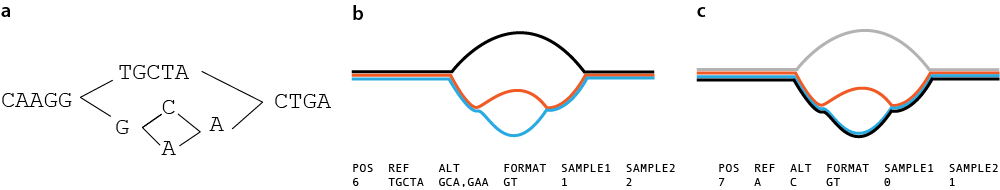
\includegraphics[width=0.95\columnwidth]{Chapter0/Figs/variant_representation.png}
\caption{{An illustration of how the...
{\label{fig:var-representation}}
}}
\end{center}
\end{figure}

\begin{figure}
\centering
\missingfigure{reference bias figure 1b in pandora paper}
\caption{A missing figure}
\label{fig:reference-bias}
\end{figure}


% =============================================
\section{\ont{} sequencing}
A description of how this sequencing technology works.

Basecalling and historical progress in accuracy. %Make sure to mention some elements like NNs that are relevant to tubby

Discuss benefits over Illumina - i.e., portability, low startup requirements, real-time results etc.

\subsection{Variant calling}
\label{sec:ont-var-calling-intro}
Variant calling - discuss history of nanopolish and recent works on variant calling such as Clair and others

% =============================================
\section{Tuberculosis and its causative agent}

Overview of the diseases and bug.

What diagnostics are available, when and how are they used

Clinically relevant applications for WGS to TB

Transmission clustering - history of this work up to "Beyond the SNP threshold"

AMR - history of this work up to mykrobe and cryptic

\subsection{Using genome graph for drug resistance prediction}
\label{sec:genome-graphs-dst}

% \drprg{} is not the first tool to use the concept of genome graphs for AMR prediction. mykrobe, the other tool used in this chapter, uses population genome graphs for genotyping of samples. The underlying method mykrobe uses is Cortex \cite{iqbal2012} - a program that uses coloured de Bruijn graphs (dBGs) for genotyping samples via \denovo{} assembly. Cortex is somewhat of a precursor to \pandora{} - the genome graph method underpinning \drprg{}. However, \pandora{} offers a number of advantages over Cortex (see \autoref{sec:genome-graphs-dst} for a full description of these). The first being the representation of the genome graph itself. As mentioned, Cortex uses \kmer{}s in coloured dBGs, while \pandora{} uses minimizing \kmer{}s in a \emph{directed} graph. In the context of \ont{} data, this distinction is important. As we saw in \autoref{chap:denovo}, build dBGs from \ont{} creates very complex graphs. In addition, as the \ont{} error rate is higher than Illumina, a smaller \kmer{} size is required, another factor that increases the complexity of the dBG. Another important difference in the graph representations of Cortex (mykrobe) and \pandora{} (\drprg{}) is the way in which \kmer{} "hits" are encorporated. In a dBG, anywhere that a \kmer{} matches, the depth is incremented by one. However, in \pandora{} such hits are dependent on the context of the read. If a \kmer{} matches two locations in the graph, but one location has many hits close by from the same read while the other does not, the spurious hit is discarded. This filtering of \kmer{} hits allows us to use a lower \kmer{} size ($k=15$) in \pandora{}, and thus \drprg{}, than is used by Cortex/mykrobe ($k=21$). Another flow-on effect of using a smaller \kmer{} size is we do not require as much read depth in \drprg{} as there is a much higher chance of matches to smaller \kmer{}s, especially when the error rate is high. For example, assuming a \ont{} error rate of 0.08, we would expect the probability of a $15-mer$ and $21-mer$ having no errors to be 0.30 and 0.19 respectively. A more in-depth discussion of the differences between these graph methods can be found in (LINK\todo{link to intro section discussing cortex/pandora differences}).

% =============================================
\section{Executive summary of this thesis}

Here I will given an overview of what things we address in each chapter